% begin module 



\begin{frame}\frametitle{The volume of a washer of thickness $dy$}

\begin{columns}[c]
\column{.5\textwidth}

$ R: $ \textbf{Outer radius} : Distance from the axis to the outer edge of the washer)\\[4mm]

$ r: $ \textbf{Inner radius} : Distance from the axis to the inner edge of the washer (radius of the "hole" in the middle)\\

%\[
%V=\alert<handout:0| 2>{\pi R^2 dy} - \alert<handout:0| 3>{\pi r^2 dy}= \pi\left(R^2-r^2\right)dy 
%\]
\column{.5\textwidth}
{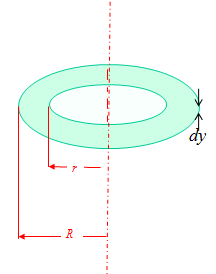
\includegraphics[height=.5\textheight]{volumes/pictures/W1}}
\end{columns}
\begin{center}

\[
\begin{array}{rcccc}
V  & =& \text{ \alert<handout:0| 2> {Volume of the disk}}&  -& \text{\alert<handout:0| 3>{Volume of the hole}.}\\[3mm]
   & =& \alert<handout:0| 2>{\pi R^2 dy} &-& \alert<handout:0| 3>{\pi r^2 dy}\\[3mm]
   & = &\pi\left(R^2-r^2\right)dy&&
\end{array}
\]
% \alert<handout:0| 2> {Volume of the disk} - \alert<handout:0| 3>{Volume of the hole}.

\end{center}
\end{frame}


\begin{frame}

\begin{example}
The region bounded by $ y=x^2 $ and $ y=2x$ is revolved about the y-axis. Find the volume.\\

\begin{columns}[c]
\column{.5\textwidth}
\uncover<2->{ We use a horizontal slice. Revolving it  makes it a ``washer".\\
The volume of the washer is
\[
V=\left(\pi R^2-\pi r^2\right)\cdot dy 
\]

$ R= $ outer radius $ = \sqrt{y}$.\\ 
$ r= $ inner radius $ = \frac{y}{2}$.\\
} %
\begin{align*}
\uncover<3->{ 
V& =\int_0^4\pi\left(\sqrt{y}^2-\left(\frac{y}{2}\right)^2 \right) \; dy\\ } %
\uncover<4->{ &=\pi \int_0^4 y-\frac14y^2\;dy\\}
\uncover<5->{ & = \pi\left[\frac{y^2}{2}-\frac{y^3}{12}\right]_0^4=\pi\cdot(8-\frac{16}{3})=\frac{8\pi}{3}
}
\end{align*}
\column{.5\textwidth} 
{\includegraphics<1>[width=.4\textwidth]{volumes/pictures/Washer1}}
{\includegraphics<2->[width=.4\textwidth]{volumes/pictures/Washer2}}
{\includegraphics<2->[width=.4\textwidth]{volumes/pictures/Washer3}}
\end{columns}
\end{example}

\end{frame}

\begin{frame}
\frametitle{Washer: Always perpendicular to the axis of rotation}
Horizontal axis of rotation:
$\ds 
V=\pi \int_a^b \left( \left[R(x)\right]^2-\left[r(x)\right]^2\right)dx
$

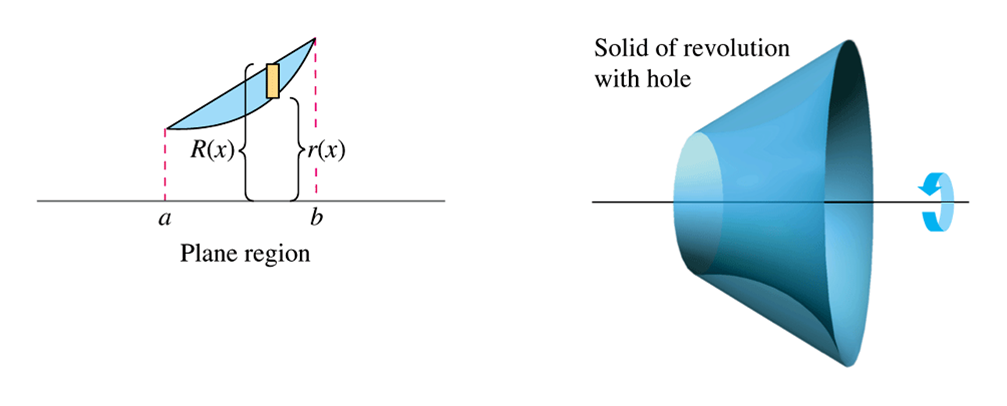
\includegraphics[height=.3\textheight]{volumes/pictures/horizontal}
%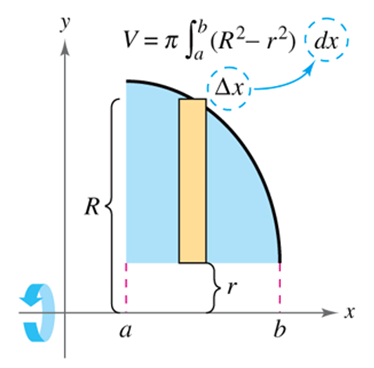
\includegraphics[height=.3\textheight]{volumes/pictures/horizontal2}

\pause 
Vertical axis of rotation:
$\ds 
V=\pi \int_c^d \left( \left[R(y)\right]^2-\left[r(y)\right]^2\right)dy
$
\includegraphics[height=.3\textheight]{volumes/pictures/vertical2}


\end{frame}





\begin{frame}

\begin{example}
The region bounded by $ y=x^2 $ and $ y=2x$ is revolved about the line $ x=2 $. Find the volume.\\
\begin{columns}[t]
\column{.5\textwidth}
\uncover<2->{\textbf{Solution:\\} Vertical axis: horizontal slice.
}
 %
\begin{align*}
\uncover<2->{
V&=\int_0^4\pi \left(R^2-r^2\right)\cdot dy\\ } 
\uncover<8->{ 
& =\int_0^4\pi\left((2-\frac{y}{2})^2-\left(2-\sqrt{y}\right)^2 \right)  dy\\ } %
\uncover<9->{ &=\pi\int_0^4 (-3y+\frac14y^2+4y^{\frac12})dy
\\}
\uncover<10->{ & = \pi\left[\frac{-3y^2}{2}+\frac{y^3}{12}+\frac83 y^{3/2}\right]_0^4\\
&=\pi\cdot(-24+\frac{16}{3}+\frac{64}{3})=\frac{8\pi}{3}
}
\end{align*}
\column{.5\textwidth} 

{\includegraphics<1>[height=.4\textheight]{volumes/pictures/same1}}
{\includegraphics<2>[height=.4\textheight]{volumes/pictures/same2}}
{\includegraphics<3>[height=.4\textheight]{volumes/pictures/same3}}
{\includegraphics<4->[height=.4\textheight]{volumes/pictures/same4}}
{\includegraphics<4->[height=.3\textheight]{volumes/pictures/same5}}
\uncover<4->{
 $ y=2x\Rightarrow x=\frac{y}{2} $.\\
$ y=x^2\Rightarrow x=\sqrt{y} $\\
}
\uncover<5->{
outer radius:} 
\uncover<6->{$ R = 2-\frac{y}{2}$.\\} 
\uncover<5->{ inner radius:}
\uncover<7->{ $ r = 2-\sqrt{y}$.\\
}
\end{columns}
\end{example}

\end{frame}

